
\paragraph{Methods}
\hfill

\subparagraph{Previous model} (Brzosko, 2017)

\noindent\textbf{Task}
\hfill \break
\noindent The environment in which the agent moves is a square field, with dimensions $4.0\times 4.0$ a.u. (arbitrary unit).
The position is encoded as $x(t)=(x, y)$, and its update $\Delta x(t)$ is defined by an action $a(t)$, represented by an angular direction $\theta$. When the agent hits a boundary $L_{\max}$, the position update is defined as a distance $d=0.01$ in the opposite direction $u(x(t))$ with respect to the boundary.

\begin{equation}
\begin{aligned}
\Delta x(t)&=
\begin{cases}   
a(t) & \text{if } x(t+1)<L_{max},\\
d\cdot u(x(t)) & \text{otherwise},
\end{cases} \\
x(t+1)&= x(t) + \Delta x(t)
\end{aligned}
\end{equation} 

\noindent Further, the connections between boundary place cells and action cells oriented outside the environment have weight of zero.
The only plastic connections are those between PCL and
AC, and the policy learned by the agent is a direct mapping between the internal spatial representation and the action space. 
\vspace{0.25cm}

\noindent\textbf{Architecture}
% brief description of the previous model
\hfill \break
\noindent The input to the model is the position vector $x(t)$ above, which can be seen as a projection from the medial entorhinal cortex (MEC) to the hippocampus (HP). This input is received by a place cells layer (PC) organized as a grid of $11\times 11$ units, and whose neural dynamics are
described by a rate model with a 2D Gaussian tuning function:

\begin{equation}
    \lambda^{pc}_{i}(x(t)) = \bar{\lambda}^{pc}\exp\left(-\frac{||x(t)-x_{i}||^{2}}{\sigma^2}\right)
\end{equation}

\noindent
where $x_{i}$ is the center of the $i$-th place cell, $\bar{\lambda}^{pc}$ is the mean firing rate set at $400$Hz, and $\sigma$ is the standard deviation of the Gaussian set at $0.4$au. This component can be identifies with the hippocampus CA1 area (\# to expand \#).
\vspace{0.25cm}

\noindent\textbf{Action cells}
\hfill \break
\noindent The PC in turn projects to a ring network of $40$ action neurons (AC) mapping directly to behavioural responses, defined as a direction angle \\ $a_{i}=a_{0}(\sin(\theta_{i}), \cos(\theta_{i}))$, where $\theta_{i}$ is the angle of the $i$-th action cell, and $a_{0}$ is a scaling parameter.
Further, the action network has a lateral inhibition mechanism, which is implemented by a Mexican hat connectivity profile, ensuring that only one action cell is active at a time.
\\ The neural
model of these cells is a Spike Response Model (SRM) (Gerstner, 2005), which is a type of rate neuron whose structure is the composed of various filters, for gating the input, the output, the refractory period, and so on. Here, the neurons have been made spiking by using the rate as a spike
probability.
\vspace{0.25cm}

\begin{figure}[ht]
    \centering
    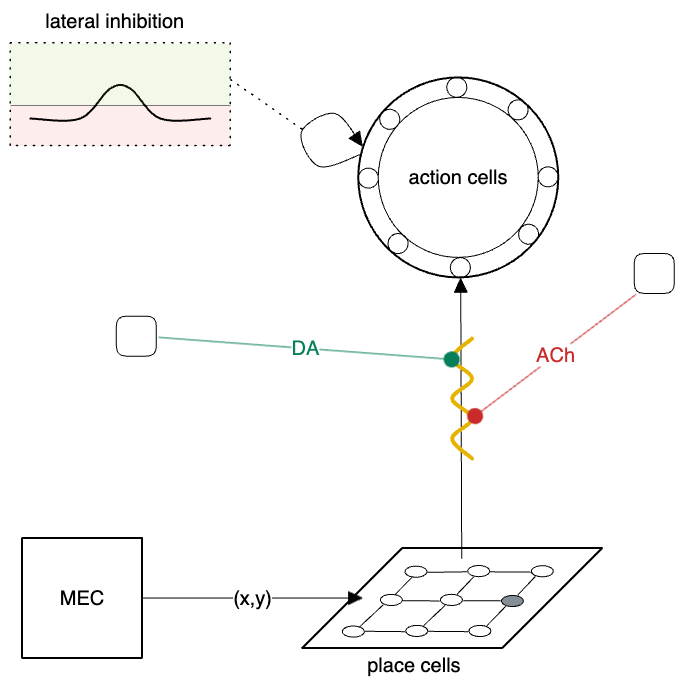
\includegraphics[scale=0.3]{figures/model_brzosko_architecture.png} 
    \caption{\textbf{Model architecture} - the input position activates a place cell, which in turn activates an action cell. The synaptic weights between the two layers are plastic and are updated by a learning rule defined in terms of dopamine (DA) and acetylcholine (ACh). The action cell network
    has lateral inhibition.}
    \label{fig:model_2}
\end{figure}

% learning
\noindent\textbf{Learning}
\hfill\break
\noindent It has been implemented as an STDP rule, empowered by a modulatory mechanism mediated by dopamine (DA) and acetylcholine (ACh). The rule for updating the synaptic weights is given by:
\begin{equation}
    \Delta w_{ij}(t)=\eta\,A\,\left(\int\limits_{-\infty}^{T^s_i}\int\limits_{-\infty}^{T^s_j}\kappa(t_i-t_j)\,dt_j\,dt_i\right)\circ \psi(t, DA)
\end{equation}\
where $w_{ij}$ is the synaptic weight between the $i$-th PCL and the $j$-th AC, $\eta$ is the learning rate, $A$ is the amplitude of the STDP window whose sign is dependent on the levels of ACh, $\kappa(t)$ is the STDP kernel, $T^s_i$ is the spike time of the $i$-th PCL, and $\psi(t, DA)$ is the
modulatory term dependent on the DA concentration.

% previous results

\begin{figure}[ht]
    \centering
    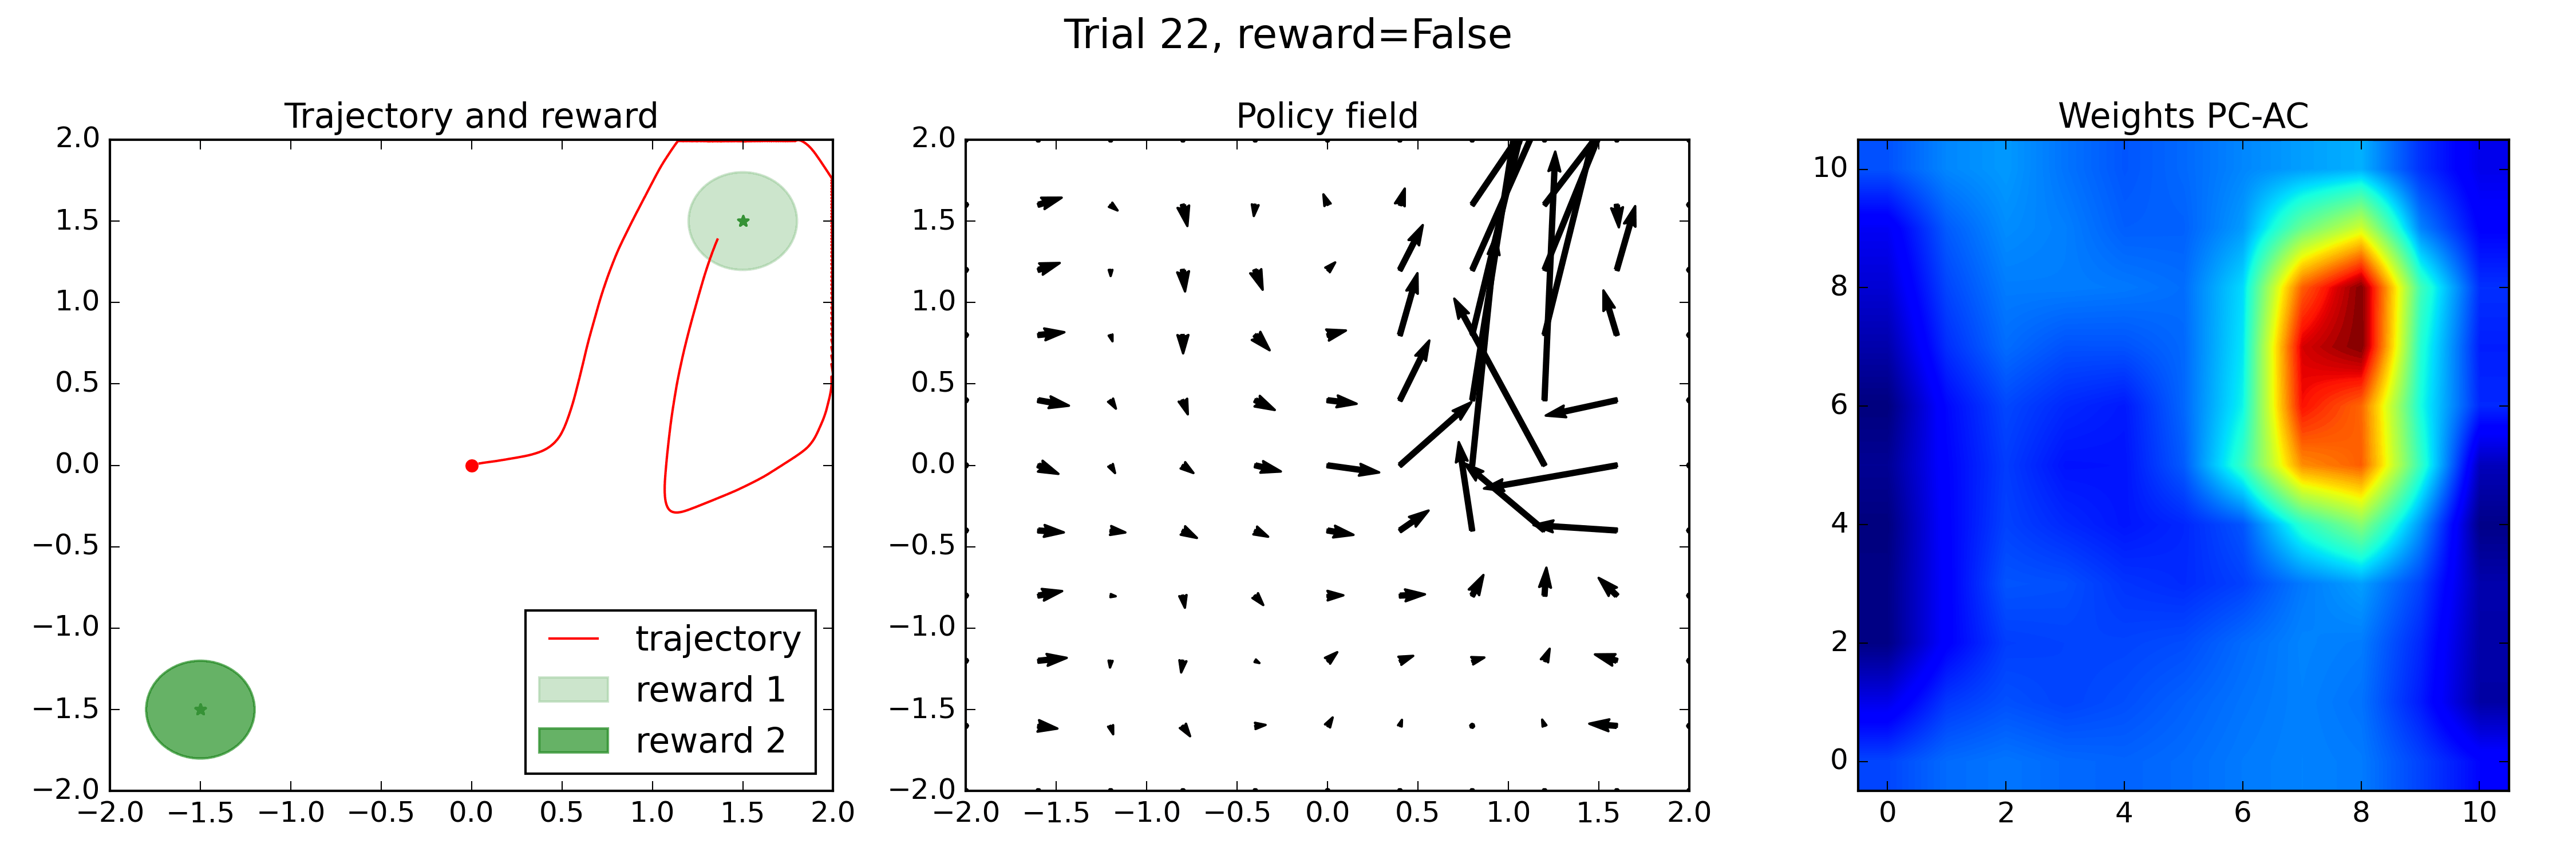
\includegraphics[scale=0.07]{figures/model_brzosko_1.png} 
    \caption{\textbf{Simulation of the agent reaching reward locations} - \textit{panel A}: the agent has successfully reached the first reward, but that has not changed to the second location; \textit{panel B}: vector field view of the agent's policy for every position in the environment;
    \textit{panel C}: reshaped and color-graded picture of the weight matrix between the place cells and the action cells.}
    \label{fig:model_1}
\end{figure}

\vspace{0.25cm}
\noindent
This model is able to learn a rewarded location and un-learn it when the reward is moved to a different location, thanks to the action of acetylcholine. However, since the policy is learned as a direct mapping between the place cells and the action cells, the memory of previous location is
inevitably overwritten. 

\subparagraph{New model}
\hfill \break
\noindent The proposed model is an extension of the previous one with a memory component, which allows the agent to remember the past reward locations.  

\hfill \break
\noindent\textbf{Task} \\
\noindent The environment is the same as before, but now with a reward association task. Initially, the agent navigates the environment randomly. Occasionally, it passes through areas where it may receives a cue (\textit{e.g.} a light) and also a reward. Its goal is to form an association between
the cue and its current position, such that it is able to to retrieve the correct reward location when it experiences the cue elsewhere. 

\hfill \break
\noindent\textbf{Architecture}\\
\noindent The input to the model is a spatial input, \textit{i.e.} the current position $x(t)$ as before, and a context $z(t)$ representing the contextual cue from the lateral entorhinal cortex (LEC). These inputs are then delivered to two distinct structures. One is a memory component, representing
CA3, which is composed of a place cells layer and an auto-associative (recurrent) network. The goal of CA3 is to form a memory trace in the recurrent synapses, binding the position and the cue. Importantly, the memory is consolidated solely in case of reward, information delivered by a dopaminergic
signal. The other structure is another place cells layer, representing the CA1, whose inputs are the current position from MEC and the retrieved position from CA3. The output of CA1 is the action cells layer. \\
The neural models are similar to before, with the only difference that for the auto-associator in CA3 the SRM equations are adapted for a balanced network of excitatory and inhibitory neurons. 

\hfill \break 
During \textit{online} navigation, the agent uses only the current position to select the action, as before, giving priority to the feedfoward connection from MEC to CA1. When the agent experiences the cue, the context is delivered to CA3, which triggers the retrieval of the associated position. This is
then delivered to CA1, which selects the action by using the angle between the two positions. Then, the agent starts a phase of \textit{offline} navigation, where the retrieved memory trace is maintained active in CA3 through a working memory mechanism. This allows it to keep selecting the action
that would lead to the reward while it is moving. 


\begin{figure}[ht]
    \centering
    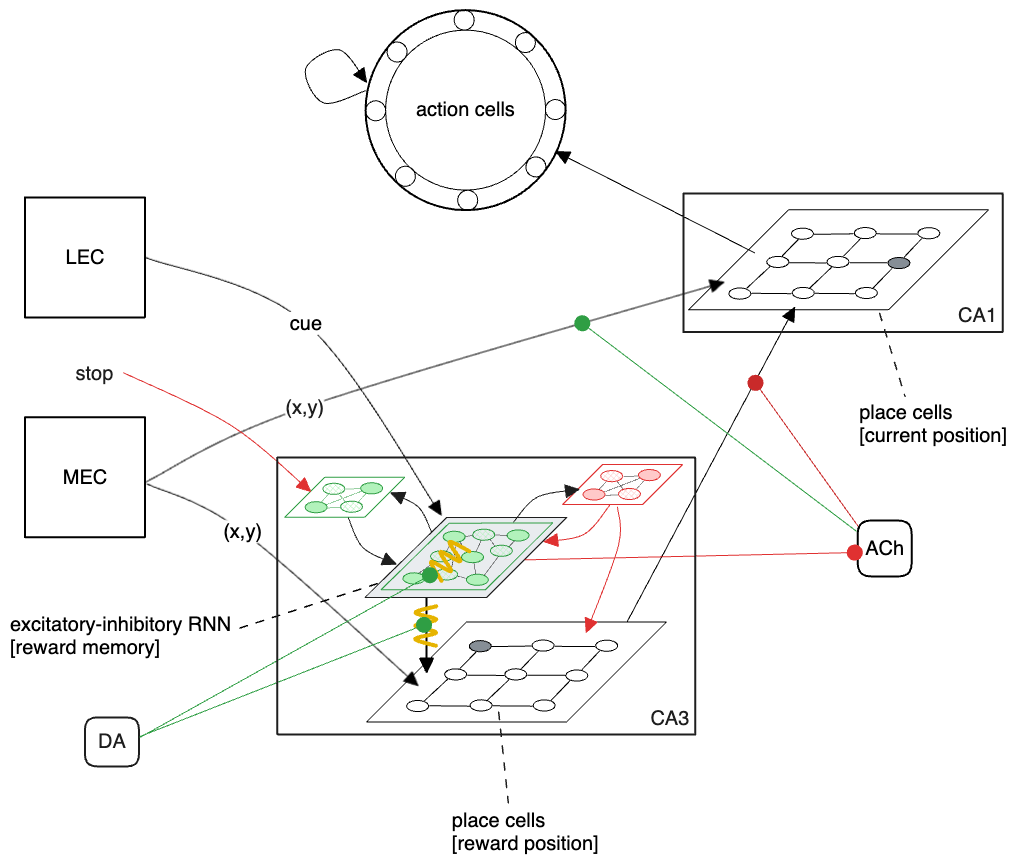
\includegraphics[scale=0.25]{figures/model_architecture.png} 
    \caption{\textbf{Model architecture} - \# write caption \#}
    \label{fig:model_3}
\end{figure}

